\documentclass[class=article, crop=false]{standalone}

\begin{document}
\section{Partie 2 - Modélisation}
\paragraph{États}À la suite de cette exercice on utilisera la notation suivant pour les états du système utilisés pour résoudre le système:
\begin{equation}\label{eq:def_states}
    X(t) =
    \begin{bmatrix}
        x_1(t)\\
        x_2(t)\\
        x_3(t)\\
        x_4(t)\\
    \end{bmatrix}
    =
    \begin{bmatrix}
        r(t)\\
        \dot{r}(t)\\
        \theta(t)\\
        \dot{\theta}(t)\\
    \end{bmatrix}
\end{equation}
\subsection{Question 4}
\begin{exercise}
    Montrer que la dynamique du système s'écrit sous forme d'état:
    \begin{equation}
        \begin{dcases}
            \frac{\text{d}}{\text{dt}} x_1(t) = x_2(t)\\
            \frac{\text{d}}{\text{dt}} x_2(t) = \frac{x_1(t) \cdot x^2_4(t) - g \cdot \sin(x_3(t))}{1 + \sigma}\\
            \frac{\text{d}}{\text{dt}} x_3(t) = x_4(t)\\
            \frac{\text{d}}{\text{dt}} x_4(t) = \frac{u(t) - m \cdot g \cdot x_1(t) \cos(x_3(t)) - 2 m \cdot x_1(t) \cdot x_2(t) \cdot x_4(t)}{J_p + m \cdot x^2_1(t)}\\
        \end{dcases}
    \end{equation}
\end{exercise}
\begin{resolution}
    On note, par la définition des coordonnés d'état, qui les états suivants sont triviales:
    \begin{equation*}
        \boxed{\frac{\text{d}}{\text{dt}} x_1(t) = x_2(t)}
        \qquad
        \boxed{\frac{\text{d}}{\text{dt}} x_3(t) = x_4(t)}
    \end{equation*}

    Ensuite, si on part de l'Équation (\ref{eq:def_Lagrange1}) en faisant la substitution des variables dynamiques pour les variables d'état on aura:
    \begin{align*}
        (1 + \sigma) \cdot \frac{\text{d}}{\text{dt}} x_2(t) 
        &= 
        x_1(t) \cdot x^2_4(t) - g \cdot \sin(x_3(t))\\
        \Aboxed{
            \frac{\text{d}}{\text{dt}} x_2(t) 
            &= 
            \frac{x_1(t) \cdot x^2_4(t) - g \cdot \sin(x_3(t))}{(1 + \sigma)}
        }
    \end{align*}

    Finalement, si on part de l'Équation (\ref{eq:def_Lagrange2}) en faisant la substitution des variables dynamiques pour les variables d'état on aura:
    \begin{align*}
        \frac{\text{d}}{\text{dt}} (J_p + m \cdot x^2_1(t)) \cdot x_4(t)
        &= 
        -m \cdot g \cdot x_1(t) \cdot \cos(x_3(t)) + u(t)
        \\
        J_p \frac{\text{d}}{\text{dt}} x_4(t) + 
        m \frac{\text{d}}{\text{dt}} (x^2_1(t) \cdot x_4(t))
        &= 
        \\
        J_p \frac{\text{d}}{\text{dt}} x_4(t) + 
        2 m \; x_1(t) \; x_2(t) \; x_4(t) +
        m \; x^2_1(t) \frac{\text{d}}{\text{dt}} x_4(t)
        &= 
        \\
        (J_p + m \; x^2_1(t)) \frac{\text{d}}{\text{dt}} x_4(t)
        &= 
        u(t) - m \; g \; x_1(t) \; \cos(x_3(t)) - 2 m \; x_1(t) \; x_2(t) \; x_4(t)
        \\
        \Aboxed{
            \frac{\text{d}}{\text{dt}} x_4(t) 
            &= 
            \frac{u(t) - m \; g \; x_1(t) \; \cos(x_3(t)) - 2 m \; x_1(t) \; x_2(t) \; x_4(t)}{(J_p + m \; x^2_1(t))}
        }
    \end{align*}
\end{resolution}

\newpage
\subsection{Question 5}
\begin{exercise}
    Modéliser le système dans le module Simulink de MATLAB. On prendra les valeurs suivantes pour les paramètres du système:
    \begin{equation}
        \begin{dcases}
            J_p &= 0.02 \; \unit{kg.m^{2}}\\
            m &= 0.6 \; \unit{kg}\\
            \sigma &= 0.8\\
            g &= 9.81 \; \unit{ms^{-2}}\\
        \end{dcases}
    \end{equation}
\end{exercise}
\begin{resolution}
    Après obtenir les équations de la dynamique du système sous forme d'état le système suivant a était mise en place en Simulink pour modéliser les équations:
    \begin{figure}[H]
        \centering
        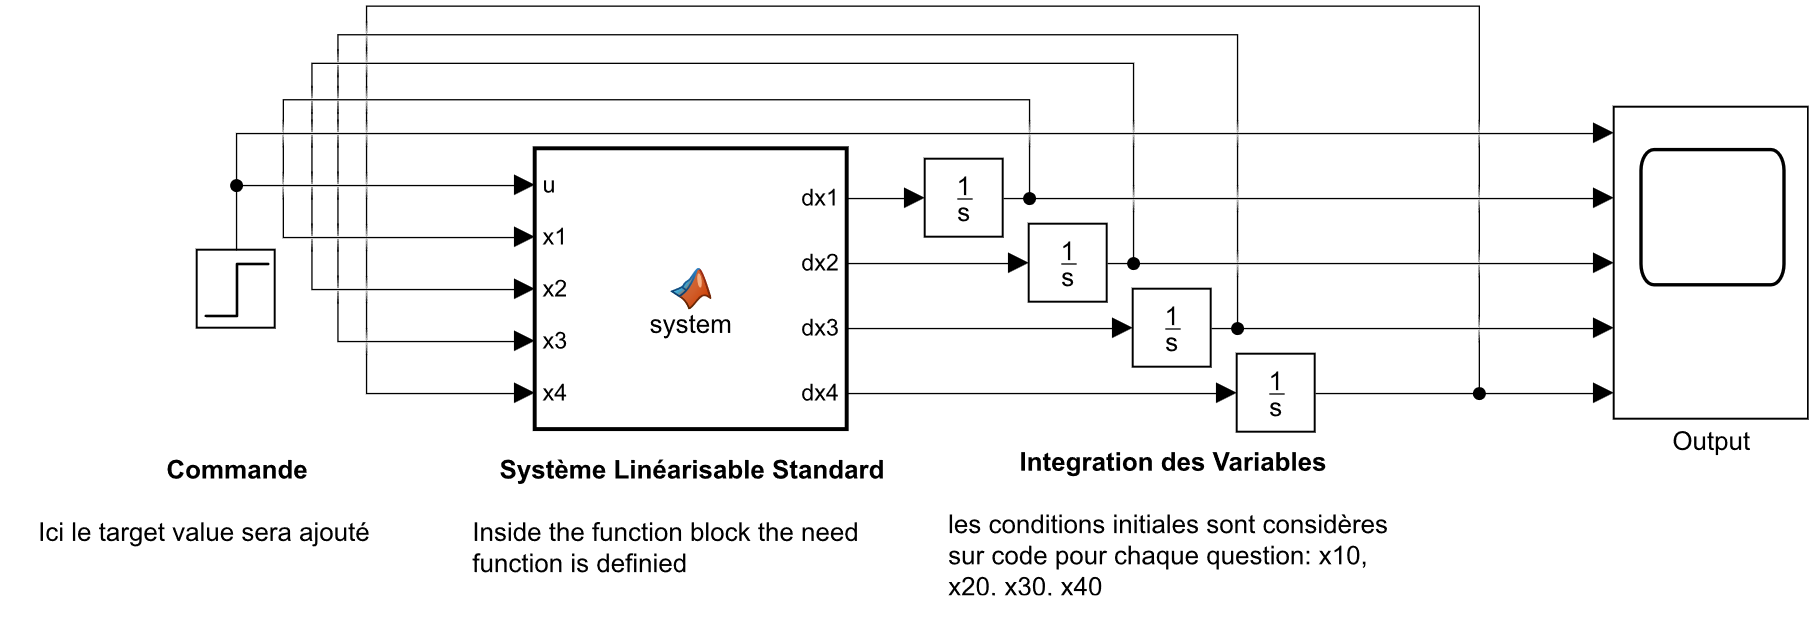
\includegraphics[width = 0.8\textwidth]{../images/system_simulink_2.png}
        \caption{Système d'Intéresse en Simulink, System}
        \label{fig:simulink_system}
    \end{figure}
    En utilisant le code suivant pour initialiser les variables nécessaires:
    \begin{scriptsize}\mycode
        \lstinputlisting[language=Matlab]{../src/Q5.m}
    \end{scriptsize}
    Dedans le bloque que represent \texttt{system} on ajoute le code suivant:
    \begin{scriptsize}\mycode
    \begin{lstlisting}[language=Matlab]
function [dx1, dx2, dx3, dx4] = system(u, x1, x2, x3, x4)
    [J, m, sig, g] = Q5(); 
    
    dx1 = x2;
    dx2 = (x1*(x2)^2 - g*sin(x3))/(1+sig);
    dx3 = x4;
    dx4 = (u - m*g*x1*cos(x3) - 2*m*x1*x2*x4)/(J + m*x1^2);
        \end{lstlisting}
    \end{scriptsize}
  
    \begin{remark}
        Comme les conditions du système ne changement pas les variables ajoutés sur chaque bloque de fonction seront données pour la fonction 5.
    \end{remark}
\end{resolution}

\newpage
\subsection{Question 6}
\begin{exercise}
    Simuler la dynamique du système avec une commande nulle pour différentes conditions initiales. Que constate-t-on?
\end{exercise}
\begin{resolution}
    En utilisant le code suivant on a une commande nulle, conditions initiales nulles, pour le système:
    \begin{scriptsize}\mycode
        \lstinputlisting[language=Matlab]{../src/P2.m}
        \lstinputlisting[language=Matlab, linerange={13-13,15-15, 19-21}]{../src/main.m}
        \lstinputlisting[language=Matlab, linerange={47-48}]{../src/main.m}
    \end{scriptsize}
    Les variables \texttt{I1} et \texttt{I2} sont utilisés pour l'initialisation des bloques d'integration. Finalement on a les résultats suivants:
    \begin{figure}[H]
        \centering
        \begin{subfigure}[b]{0.475\textwidth}
            \centering
            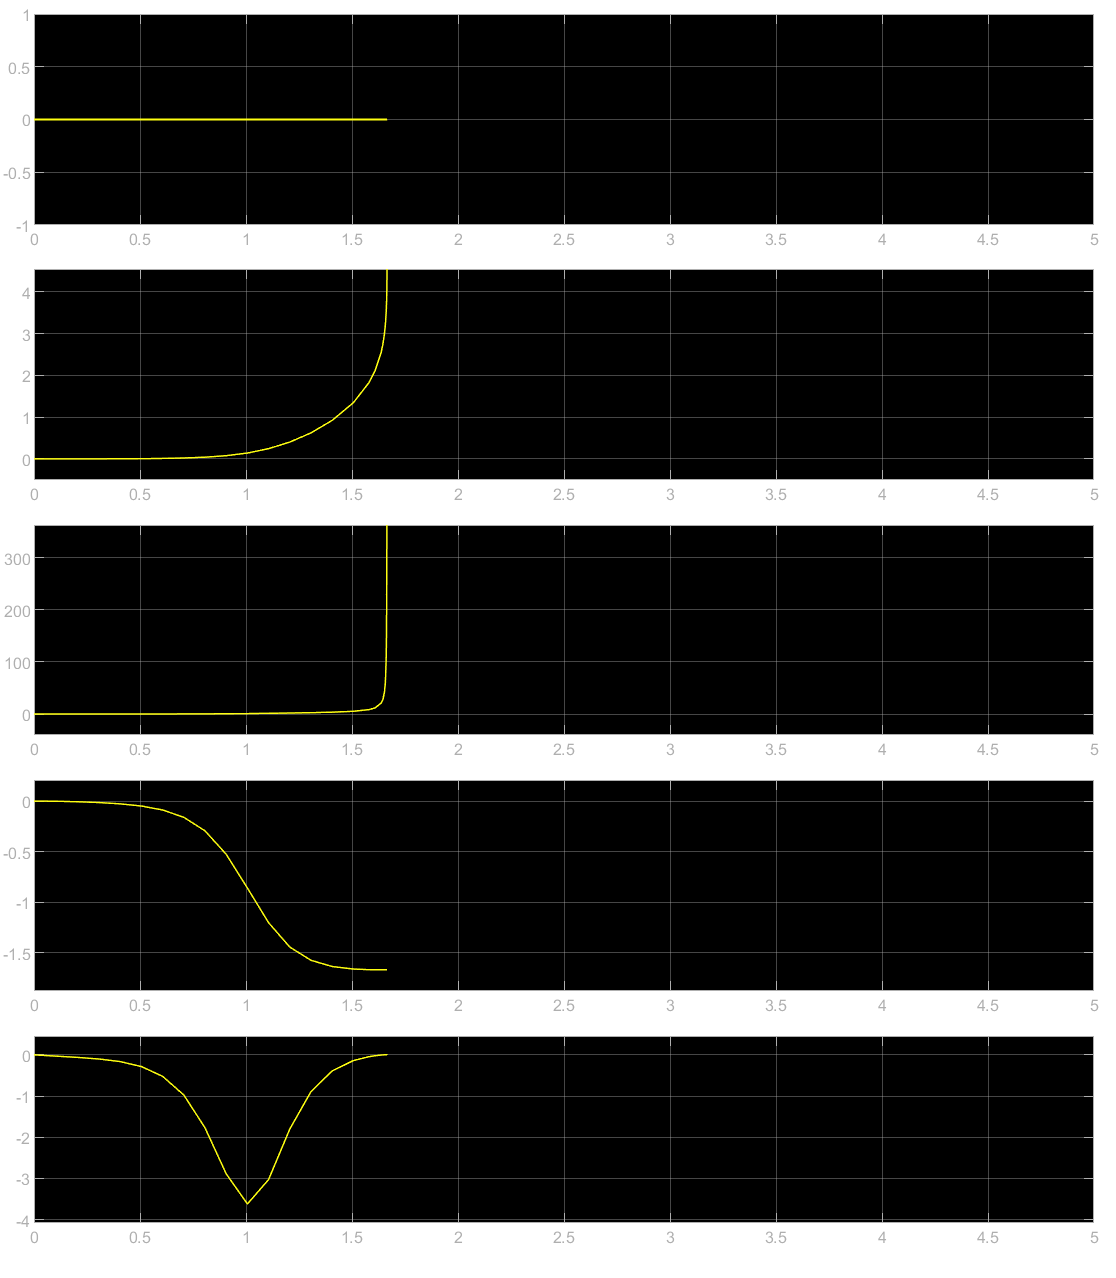
\includegraphics[width=\textwidth]{../images/simulink_scope2_0_01.png}
            \caption{with $x_1(0) = 0.001$}
        \end{subfigure}
        \begin{subfigure}[b]{0.475\textwidth}
            \centering
            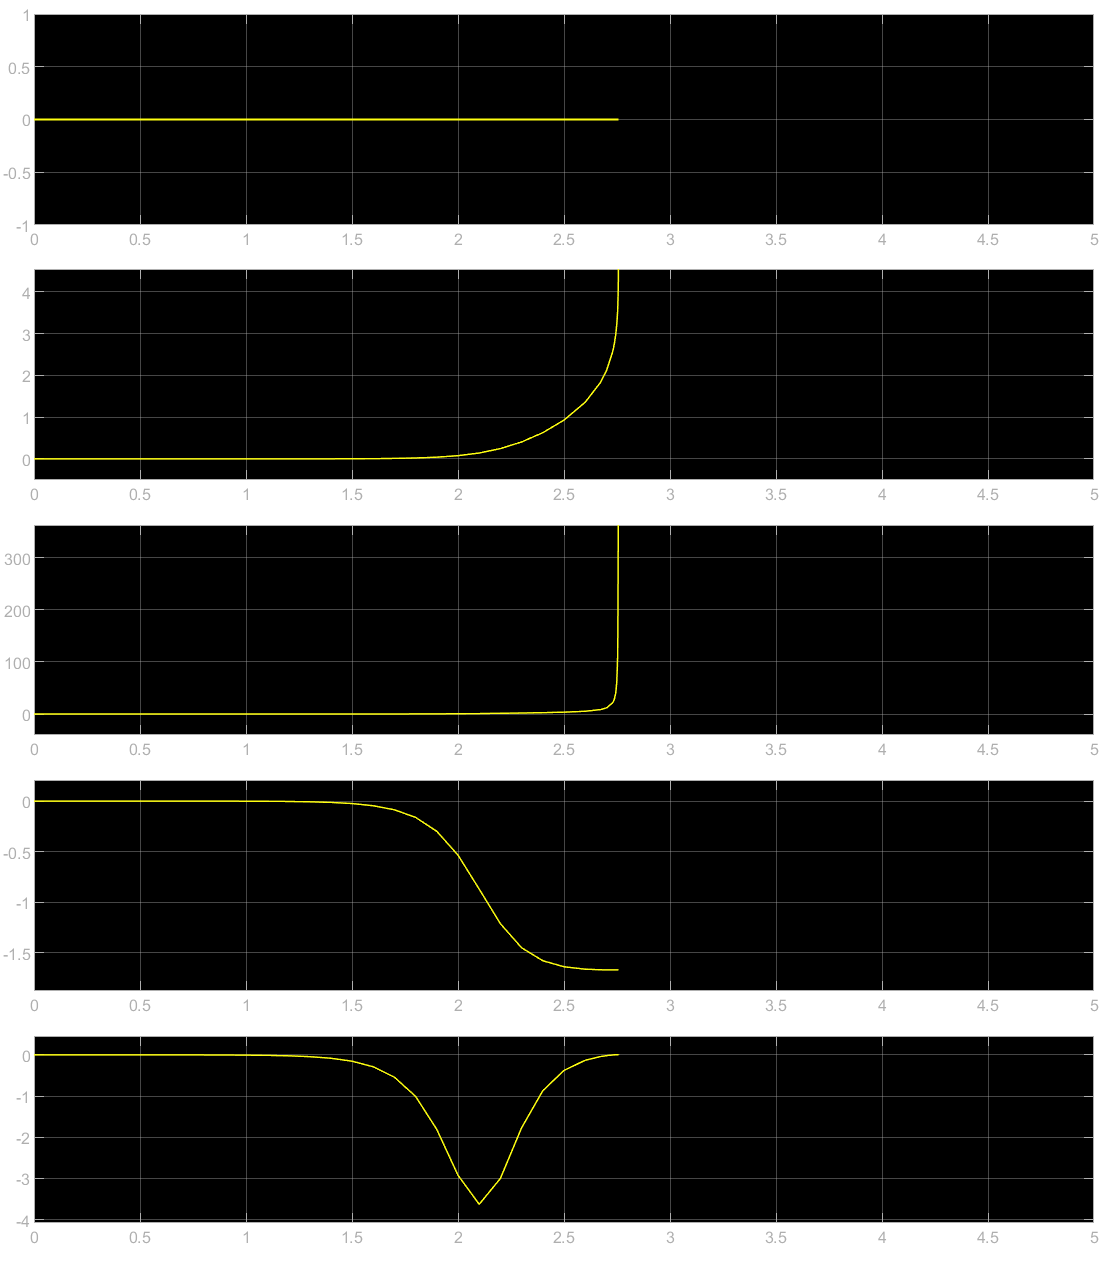
\includegraphics[width=\textwidth]{../images/simulink_scope2_0_000001.png}
            \caption{with $x_1(0) = 0.000001$}
        \end{subfigure}
        \caption{Simulation Conditions Initiales, $x_2(0) = x_3(0) = x_4(0) = 0$}
        \label{fig:simulink_simulation_conditions_initiales}
    \end{figure}
    On note que, indépendamment des variables initiales choisîtes, le système diverge après quelques instants de simulation.
    \begin{phrase}
        Dans la suite de cette rapport sur les images de simulation on considère que le premier graphique en haut sera la commande $u(t)$ et à la suite sont les état $x_1(t)$, $x_2(t)$, $x_3(t)$ et $x_4(t)$.
    \end{phrase}
\end{resolution}

\newpage
\subsection{Question 7}
\begin{exercise}
    Quels sont les points d'équilibre du système? Peut-on stabiliser la balle sur n'importe quelle position de $r_{\text{ref}}$?\\
    
Exprimer l'état d'équilibre et la commande d'équilibre en fonction de la position $r_{\text{ref}}$ sur laquelle on souhaite stabiliser la balle.
\end{exercise}
\begin{resolution}
    Si on considère une système donne pour $X(t) = f(X(t), u(t))$ l'équilibre se fait quand $f(X_e(t), u_e(t)) = 0$ donc si on considère $x_1(t) = r_{\text{ref}}$ on a:
    \begin{equation*}
        \begin{dcases}
            \frac{\text{d}}{\text{dt}} x_1(t) = 0 = x_2(t) & 
            \boxed{x_2(t) = 0}
            \\
            \frac{\text{d}}{\text{dt}} x_2(t) = 0 = \frac{ r_{\text{ref}} \; x^2_4(t) - g \; \sin(x_3(t))}{1 + \sigma} & 
            \sin(x_3(t)) = 0 \therefore \boxed{x_3(t) = 0 = 0\,[2\pi]}
            \\
            \frac{\text{d}}{\text{dt}} x_3(t) = 0 = x_4(t) & 
            \boxed{x_4(t) = 0}
            \\
            \frac{\text{d}}{\text{dt}} x_4(t) = 0 = \frac{u(t) - m \; g \; r_{\text{ref}} \cos(x_3(t)) - 2 m \; r_{\text{ref}} \; x_2(t) \; x_4(t)}{J_p + m \; r_{\text{ref}}^2} & 
            \boxed{u(t) = m \; g \; r_{\text{ref}}}
            \\
        \end{dcases}
    \end{equation*}
    Finalement on note l'état d'équilibre $X_e(t)$ sera donne pour:
    \begin{equation}
        X_e(t) = 
        \begin{bmatrix}
            x_{1_e}\\
            x_{2_e}\\
            x_{3_e}\\
            x_{4_e}\\
        \end{bmatrix}
        =
        \begin{bmatrix}
            r_{\text{ref}}\\
            0\\
            0\\
            0\\
        \end{bmatrix}
        \quad\text{e}\quad
        u_e(t) = m \; g \; r_{\text{ref}}
    \end{equation}
    On note que tous les points d'équilibre du système seront données en fonction de $r_{\text{ref}}$ si on a $X_e(t)$ et $u_e(t)$.
    \begin{remark}
        Il faut noter que pour $x_3(t)$ il y avait deux solutions possibles:
        \begin{equation*}
            \sin(x_3(t)) = 0 
            \quad
            \begin{cases}
                x_3(t) = 0\,[2\pi]\\
                x_3(t) = \pi\,[2\pi]\\
            \end{cases}
        \end{equation*}
        Où $\theta\,[2\pi]$ représente tous les positions possibles d'obtenir l'angle $\theta$ dans le circle trigonométrique.\\
        
        La réponse $x_3(t) = \pi\,[2\pi]$ représente le plateau à l'envers, avec une angle de $180^{\circ}$, qui n'a pas de signification physique pour ce système et pour cette raison n'était pas considère comme une réponse valable.
    \end{remark}
\end{resolution}

\newpage
\subsection{Question 8}
\begin{exercise}
    Ajouter dans le modèle Simulink un bloc permettant de calculer l'état d'équilibre $X_{\text{ref}}$ et la commande d'équilibre $u_{\text{ref}}$ en fonction de la position $r_{\text{ref}}$ sur laquelle on souhaite stabiliser la Balle. Vérifier avec le modèle Simulink pour différentes valeurs de $r_{\text{ref}}$ que si le système n'est pas initialisé exactement à l'équilibre, les trajectoires divergent.
\end{exercise}
\begin{resolution}
    Après obtenir les équations de l'équilibre du système la fonction suivante a était mise en place en Simulink:
    \begin{figure}[H]
        \centering
        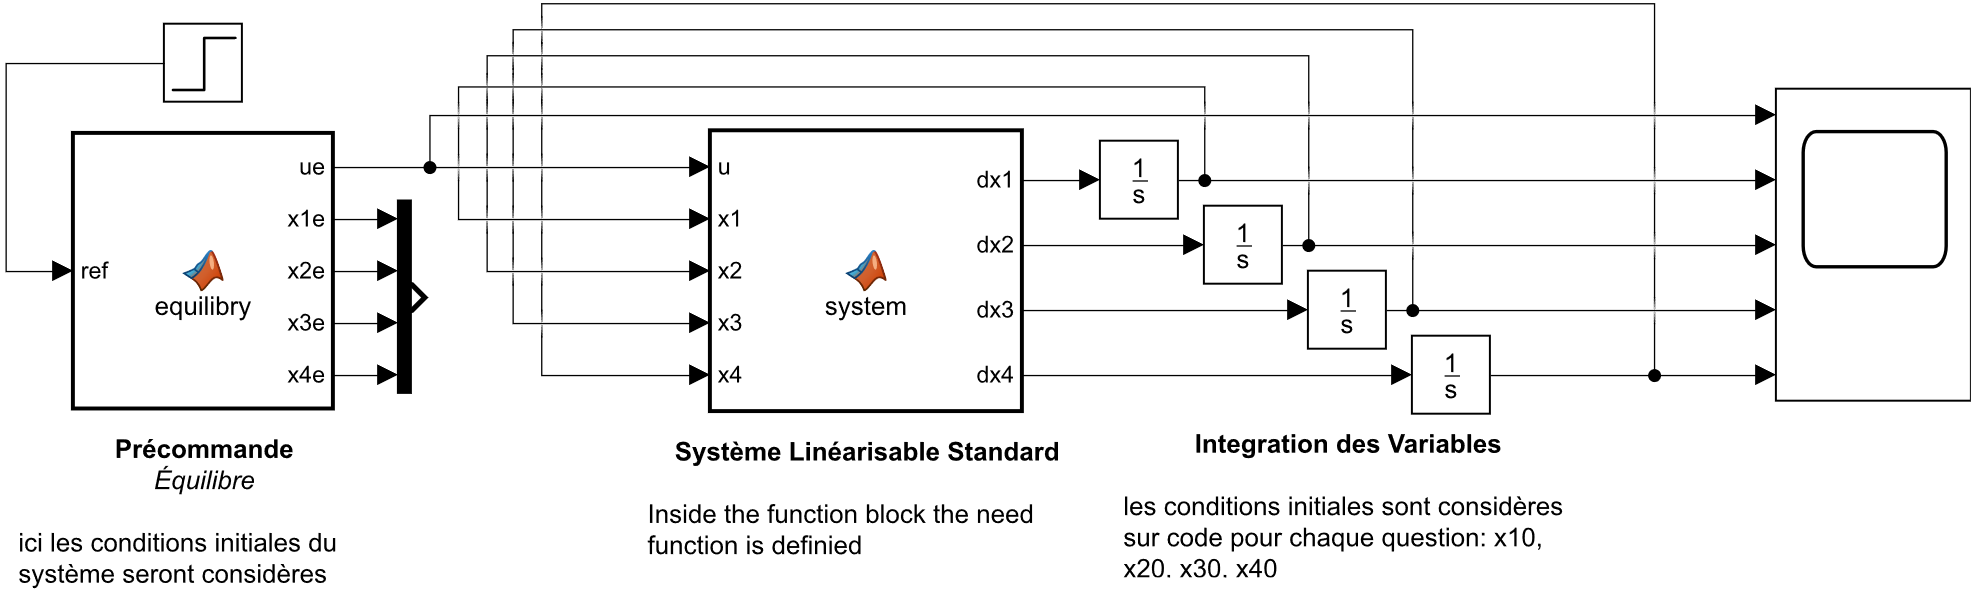
\includegraphics[width = 0.8\textwidth]{../images/system_simulink_20.png}
        \caption{Système d'Intéresse en Simulink, Équilibre}
        \label{fig:simulink_system_equilibry}
    \end{figure}
    Dedans le bloque que represent \texttt{equilibry} on ajoute le code suivant:
    \begin{scriptsize}\mycode
        \begin{lstlisting}[language=Matlab]
function [ue, x1e, x2e, x3e, x4e] = equilibry(ref)
    x1e = ref;
    x2e = 0;
    x3e = 0;
    x4e = 0;
    ue  = m*g*x1e; 
        \end{lstlisting}
    \end{scriptsize}

    Qui donne des résultats suivants:
    \begin{figure}[H]
        \centering
        \begin{subfigure}[b]{0.425\textwidth}
            \centering
            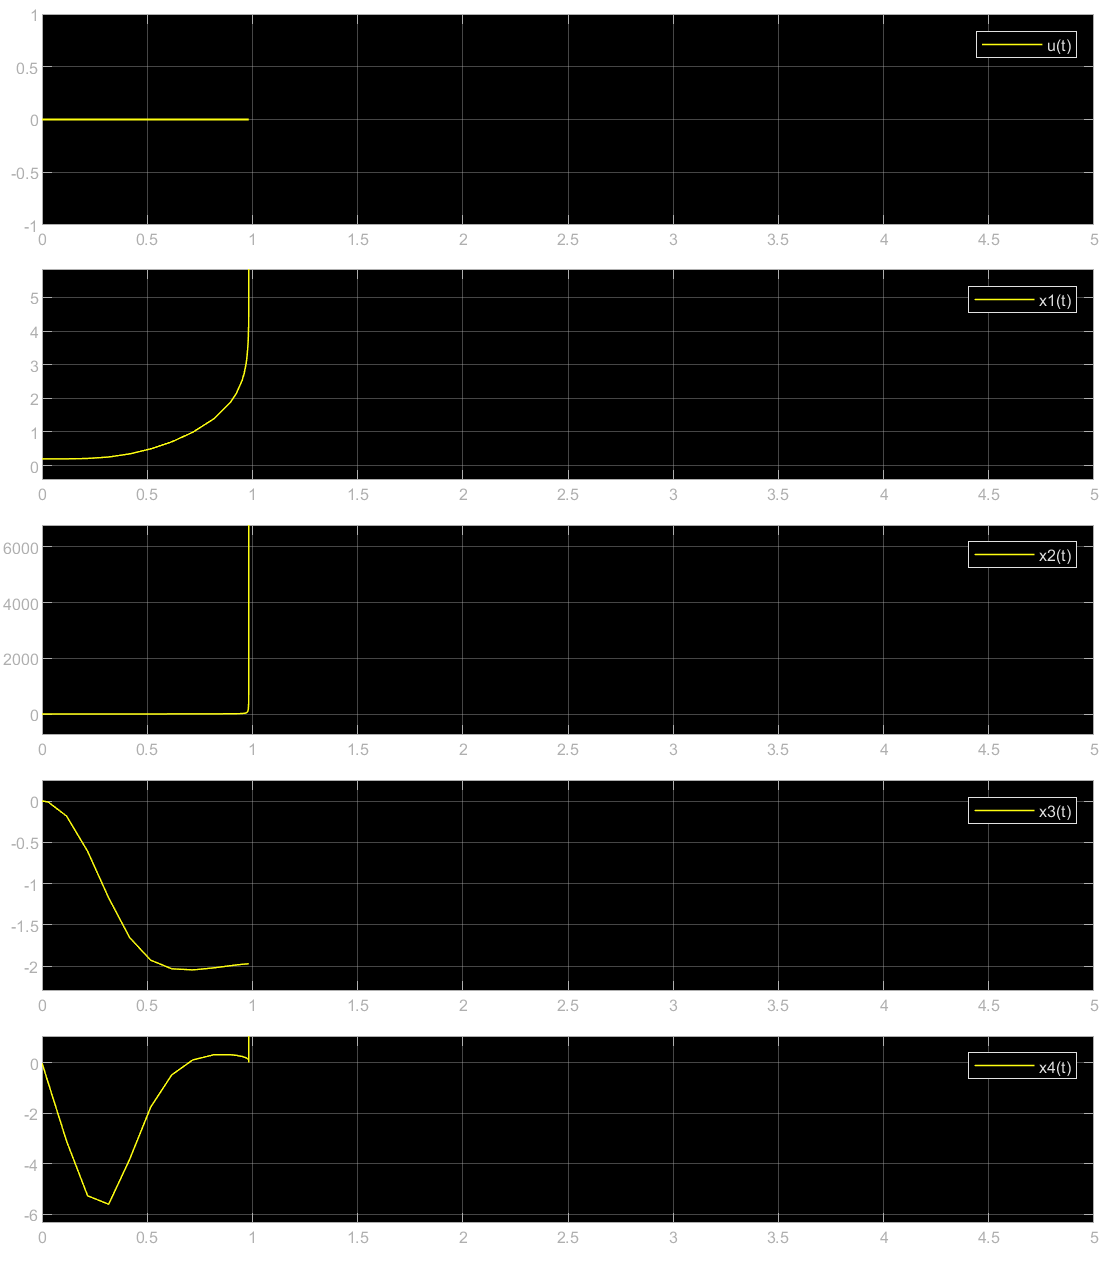
\includegraphics[width=\textwidth]{../images/simulink_scope20_02_02.png}
            \caption{with $x_1(0) = 0.2$ and $r_{\text{ref}} = 0.2$}
        \end{subfigure}
        \begin{subfigure}[b]{0.425\textwidth}
            \centering
            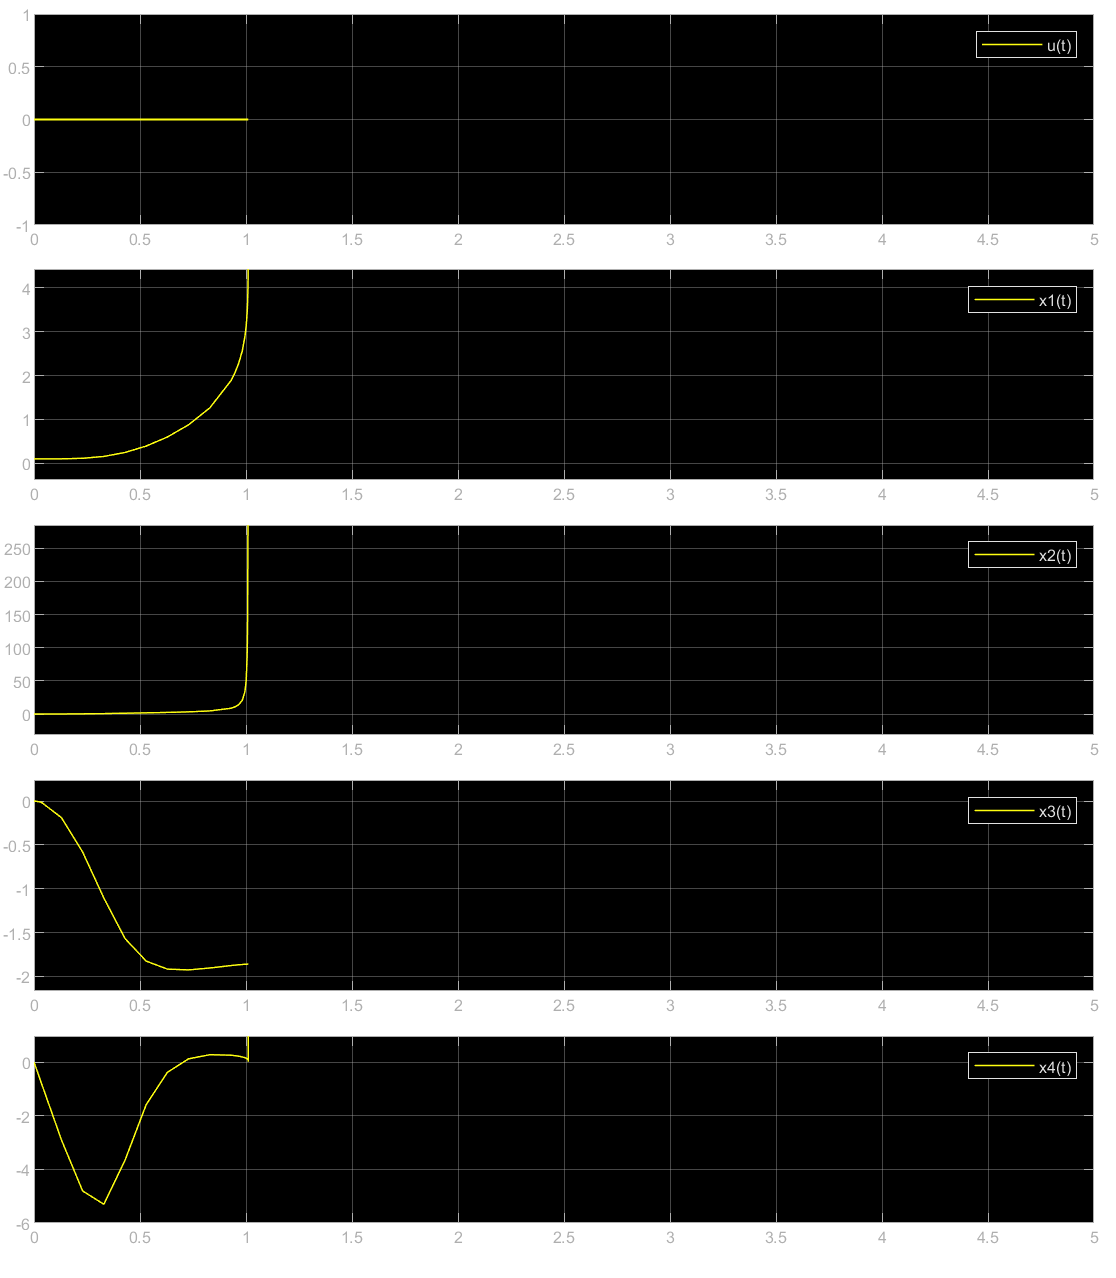
\includegraphics[width=\textwidth]{../images/simulink_scope20_02_01.png}
            \caption{with $x_1(0) = 0.1$ and $r_{\text{ref}} = 0.2$}
        \end{subfigure}
        \caption{Simulation Équilibre, $x_2(0) = x_3(0) = x_4(0) = 0$}
        \label{fig:simulink_simulation_équilibre}
    \end{figure}
    On note que, hors de l'équilibre, le système diverge comme attendu.
\end{resolution}

\newpage
\subsection{Question 9}
On note $X(t) = X_{\text{ref}} + \delta X(t)$ et $u(t) = u_{\text{ref}} + \delta u(t)$ sont les écarts à l'équilibre. On second intéresse à l'équilibre associé à $r_{\text{ref}} = 0$.
\begin{exercise}
    Montrer que le linéarisé tangent autour de la position d'équilibre $r_{\text{ref}} = 0$ s'écrit:
    \begin{equation}
        \frac{\text{d}}{\text{dt}} 
        \underbrace{
        \begin{bmatrix}
            \delta x_{1}(t)\\
            \delta x_{2}(t)\\
            \delta x_{3}(t)\\
            \delta x_{4}(t)\\
        \end{bmatrix}}_{\delta X(t)}
        =
        \underbrace{
            \begin{bmatrix}
            0 & 1 & 0 & 0\\
            0 & 0 & -\frac{g}{1 + \sigma} & 0\\
            0 & 0 & 0 & 1\\
            -\frac{mg}{J_p} & 0 & 0 & 0\\
        \end{bmatrix}}_{A}
        \underbrace{
        \begin{bmatrix}
            \delta x_{1}(t)\\
            \delta x_{2}(t)\\
            \delta x_{3}(t)\\
            \delta x_{4}(t)\\
        \end{bmatrix}}_{\delta X(t)}
        +
        \underbrace{
            \begin{bmatrix}
            0\\
            0\\
            0\\
            \frac{1}{J_p}\\
        \end{bmatrix}}_{B}
        \delta u(t)
    \end{equation}
\end{exercise}
\begin{resolution}
    On part de la solution obtenu sur la Question 7:
    \begin{equation*}
        \underbrace{
        \begin{bmatrix}
            x_1(t)\\
            x_2(t)\\
            x_3(t)\\
            x_4(t)\\
        \end{bmatrix}}_{X(t)}
        \to
        \begin{dcases}
            \frac{\text{d}}{\text{dt}} x_1(t) = x_2(t)
            \\
            \frac{\text{d}}{\text{dt}} x_2(t) = \frac{ x_1(t) \; x^2_4(t) - g \; \sin(x_3(t))}{1 + \sigma}
            \\
            \frac{\text{d}}{\text{dt}} x_3(t) = x_4(t)
            \\
            \frac{\text{d}}{\text{dt}} x_4(t) = \frac{u(t) - m \; g \; x_1(t) \cos(x_3(t)) - 2 m \; x_1(t) \; x_2(t) \; x_4(t)}{J_p + m \; x^2_1(t)}
            \\
        \end{dcases}
    \end{equation*}
    Pour la linéarisation les approximations suivants seront considères
    \begin{equation}
        \sin(\alpha) \approx \alpha
        \qquad
        \cos(\alpha) \approx 1
        \qquad
        x^2(t) \approx 0
    \end{equation}
    En plus, les termes qui ont des multiplications des états seront considères comme zéros car ils ne sont pas linéaires. C'est-à-dire que le système d'équations précédemment sera simplifier à:
    \begin{equation*}
        \underbrace{
        \begin{bmatrix}
            x_1(t)\\
            x_2(t)\\
            x_3(t)\\
            x_4(t)\\
        \end{bmatrix}}_{X(t)}
        \to
        \begin{dcases}
            \frac{\text{d}}{\text{dt}} x_1(t) = x_2(t)
            \\
            \frac{\text{d}}{\text{dt}} x_2(t) = \frac{- g \; x_3(t)}{1 + \sigma}
            \\
            \frac{\text{d}}{\text{dt}} x_3(t) = x_4(t)
            \\
            \frac{\text{d}}{\text{dt}} x_4(t) = \frac{u(t) - m \; g \; x_1(t)}{J_p}
            \\
        \end{dcases}
    \end{equation*}
    Qui en notation matricielle donnera le système suivant:
    \begin{equation*}
        \boxed{
            \frac{\text{d}}{\text{dt}} 
            \underbrace{
            \begin{bmatrix}
                \delta x_{1}(t)\\
                \delta x_{2}(t)\\
                \delta x_{3}(t)\\
                \delta x_{4}(t)\\
            \end{bmatrix}}_{\delta X(t)}
            =
            \underbrace{
                \begin{bmatrix}
                0 & 1 & 0 & 0\\
                0 & 0 & -\frac{g}{1 + \sigma} & 0\\
                0 & 0 & 0 & 1\\
                -\frac{mg}{J_p} & 0 & 0 & 0\\
            \end{bmatrix}}_{A}
            \underbrace{
            \begin{bmatrix}
                \delta x_{1}(t)\\
                \delta x_{2}(t)\\
                \delta x_{3}(t)\\
                \delta x_{4}(t)\\
            \end{bmatrix}}_{\delta X(t)}
            +
            \underbrace{
                \begin{bmatrix}
                0\\
                0\\
                0\\
                \frac{1}{J_p}\\
            \end{bmatrix}}_{B}
            \delta u(t)
        }
    \end{equation*}
\end{resolution}

\newpage
\subsection{Question 10}
On pose:
\begin{equation}
    \omega = 
    \sqrt[4]{\frac{m \cdot g^2}{(1 + \sigma) \cdot J_p}}
\end{equation}
\begin{exercise}
    Calculer les valeurs propres du linéarisé tangent en boucle ouverte en fonction de $\omega$. Le système en boucle ouverte est-il stable? Vérifier numériquement les valeurs propres en boucle ouverte avec MATLAB.
\end{exercise}
\begin{resolution}
    On part de la matrice $A$ découvert dans la Question 9 et on calcule les valeurs propres $\lambda$ avec l'équation suivante:
    \begin{equation*}
        \underbrace{
            \det (A - \lambda I) = 0
        }_{\text{valeurs propres définition}}
        \implies
        \begin{vmatrix}
            -\lambda & 1 & 0 & 0\\
            0 & -\lambda & -\frac{g}{1 + \sigma} & 0\\
            0 & 0 & -\lambda & 1\\
            -\frac{mg}{J_p} & 0 & 0 & -\lambda\\
        \end{vmatrix}
        = 0
        \xRightarrow[]{\text{\href{https://en.wikipedia.org/wiki/Laplace_expansion}{Laplace Expansion}}}
        \boxed{
            \lambda^4 = \frac{m \cdot g^2}{(1 + \sigma) \cdot J_p} = \omega^4
        }
    \end{equation*}
    Finalement les valeurs propres seront:
    \begin{equation}
        \begin{cases}
            \lambda_{1,2} = \pm \omega\\
            \lambda_{3,4} = \pm \omega \cdot i\\
        \end{cases}
        \xRightarrow[]{\omega = 6.3284}
        \begin{cases}
            \lambda_{1,2} = \pm 6.3284\\
            \lambda_{3,4} = \pm 6.3284 \cdot i\\
        \end{cases}
    \end{equation}
    En utilisant le code suivant on calcule les valeurs propres du système:
    \begin{scriptsize}\mycode
        \lstinputlisting[language=Matlab]{../src/Q10.m}
    \end{scriptsize}
    Qui retourne les valeurs suivants:
    \begin{scriptsize}\mycode
        \begin{lstlisting}[language=Matlab]
>>>
eigenValues =

    -6.3284 + 0.0000i
    -0.0000 + 6.3284i
    -0.0000 - 6.3284i
    +6.3284 + 0.0000i
    
warning: system diverge eig 6.3284
        \end{lstlisting}
    \end{scriptsize}
    On peut voir que les valeurs propres théoriques et numériques sont les mêmes.\\

    On remarque qu'une valeur propre a la partie réelle plus grand que zéro qui fait que le système soit instable comme montrer pour les Questions 6 et 8.\\
\end{resolution}
\end{document}